\documentclass[12pt,fleqn]{article}\usepackage{../common}
\begin{document}
Ders 6

Bu derste islenecek onemli konular sunlar, bir matrisin kolon uzayi
(columnspace), ki bu konuya onceki derste degindik, digeri ise bir
matrisin sifir uzayi (nullspace) ve alt uzaylar. 

Simdi alt uzaylar hakkinda bir dusunce deneyi yapalim. Diyeli ki elimde $P$
ve $L$ diye iki tane alt uzay var, $P$, $\mathbb{R}^3$ icinde bir duzlem
(plane), $L$ ise $P$ uzerinde olmayan bir cizgi (line). $P$ ve $L$ tabii ki
orijinden geciyorlar, yoksa alt uzay olmazlar. 

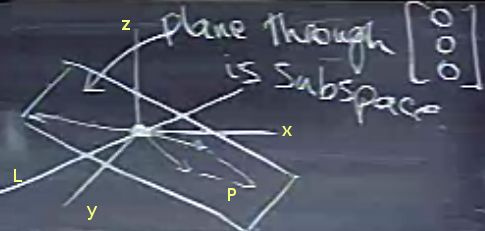
\includegraphics[height=4cm]{6_01.png}

Soru sudur; bu iki uzayin birlesimi (union) bir alt uzay olusturur mu?
Cevap hayir. Cunku belirtilen mustakbel uzay toplanabilme prensibine izin
vermiyor. Bu prensibe gore bir uzay icindeki iki vektorun toplami ayni uzay
icinde olmaliydi degil mi? Bir cizgi ve duzlemin toplami olan ``sey'' bu
tanima uymuyor. Gayet rahat bir sekilde duzlemden bir vektor, $L$'den bir
vektor alip onlari toplarsam bambaska bir yone isaret eden bir yeni vektor
elde edebilirim ve bu vektor $P \cup L$ icinde olmaz.

Peki $P \cap L$'i dusunelim, yani her iki uzayin kesisimi olan kume bir
alt uzayi midir? Kesisimde ne oldugunu dusunelim, sadece orijin noktasi
var, o zaman kumede sadece sifir noktasi var. Sifir vektoru tek basina bir
alt uzay olusturabilir mi? Evet. Bu kume bir alt uzay olusturabilir mi?
Cevap yine evet. 

Soruyu daha genellestirerek soralim: herhangi iki alt uzay $S,T$'yi alalim,
$S \cap T$ her zaman bir alt uzay olur mu? Bu alt uzay daha ufak olacaktir,
cunku sartlari daha spesifik hale getirdik, bir nokta hem $S$ hem $T$
icinde olmalidir, herhalde bu sarta uyan noktalar daha azdir. Ama cevap
yine evet. Dusunelim; kesisimden $v,w$ adli iki vektor alalim, o zaman
$u + w$, $S$ icinde mi? Evet, cunku $u,w$'nin ikisi de tanim itibariyle $S$
icinde, ve $S$ bir alt uzay olduguna gore onun icindeki iki vektorun
toplami da ayni uzay icinde olmlaya meburdur, ve ayni durum $T$ icin de
gecerlidir. Toplam demek ki hem $S$ hem $T$ icinde olacaktir, bunu
soylerken yani ``hem $S$ hem $T$ icinde'' derken ayni zamanda kesisimi
tarif etmis olmadik mi? Evet, o zaman toplam ayni zamanda kesisim icindedir
de. Ispat tamamlandi. 

Alt uzay kontrolunun ikinci ogesi neydi? Sabitle carpim yine uzay icinde
olmali. Ayni argumani kullaniyoruz, $S \cap T$ icinde olan bir vektoru
alirim, mesela 7 ile carparim, sonuc yine $S$ icinde cunku $S$ bir alt
uzaydi, $T$ icinde, ayni sebepten dolayi. Demek ki carpim hem $S$ hem $T$
icinde bu sebeple $S \cap T$ icinde.

O zaman iki alt uzayin kesisimi kesinlikle bir alt uzaydir. 

$A$'nin Kolon Uzayi

$$ A = 
\left[\begin{array}{rrr}
1 & 1 & 2 \\
2 & 1 & 3 \\
3 & 1 & 4 \\
4 & 1 & 5 
\end{array}\right]
 $$


Bu matrisin kolon uzayi $\mathbb{R}^4$'un bir alt uzayidir cunku kolondaki
vektorler 4 boyutlu. $A$'nin kolon uzayinda, ki buna $C(A)$ diyelim, ne
vardir? Ustte gordugumuz $A$'nin tum kolonlari, ucu de, oradadir. Ama bu
yeterli degil tabii ki, degil mi? 3 tane vektor koyarak bir alt uzay elde
etmis olmam. Bu alt uzayi nasil doldururum? Ustteki uc vektorun tum lineer
kombinasyonlarini alirim ve alt uzaya koyarim. Bunu yaparsam bir vektor
uzayi elde etmis olabilirim fakat hala bir alt uzay elde etmis olmam. 

Ustteki uc vektorun tum kombinasyonlari tum 4 boyutlu uzayi (yani
$\mathbb{R}^4$) doldurur mu? Cevap hayir. Yani ispatsal olarak bunu
gostermemis olsak bile sezgimiz bunun olmayacagi yonunde (ki bu sezgi
dogru). 

Fakat bu kombinasyonlar daha ufak bir uzay olacagi kesin. Ne kadar ufak? 

Bu sorunun cevabini vermek icin lineer denklemler ile bir baglanti kurmak
faydali olacak. Sorular sunlar,

``$Ax = b$ denkleminin her $b$ icin bir cozumu var midir?''

Bir diger baglantili soru, ``hangi $b$'ler icin cozum vardir?''

1. sorunun cevabi hayir; cunku elimde 4 tane denklem, ama 3 tane bilinmeyen
var, yani bazi $b$'ler icin cozumun olmamasi gayet normal. Ustteki ornegi
genisletirsek,

$$ A = 
\left[\begin{array}{rrr}
1 & 1 & 2 \\
2 & 1 & 3 \\
3 & 1 & 4 \\
4 & 1 & 5 
\end{array}\right]
\left[\begin{array}{r}
x_1  \\
x_2  \\
x_3  
\end{array}\right] 
=
\left[\begin{array}{r}
b_1  \\
b_2  \\
b_3  \\
b_4  
\end{array}\right]
 $$

Fakat ``bazi'' (esitligin) sag taraflari icin bu denklemin cozumu
vardir. Bu da 2. sorunun cevabini verecek, ilgilendigim sag taraflar
bunlar. 

En bariz $b$ hangisi? Sifir vektor. O zaman $x$'i de sifir vektor alirim,
ve bu bir cozum olur. Bir diger cozum? [Siniftan bir cevap geliyor, hoca
yaziyor]


$$ A = 
\left[\begin{array}{rrr}
1 & 1 & 2 \\
2 & 1 & 3 \\
3 & 1 & 4 \\
4 & 1 & 5 
\end{array}\right]
\left[\begin{array}{r}
x_1  \\
x_2  \\
x_3  
\end{array}\right] 
=
\left[\begin{array}{r}
1  \\
2  \\
3  \\
4  
\end{array}\right]
 $$

Bu $b$ icin cozum vardir? Hangi $x$ bu denklemi cozer? Haldir huldur hucre
hucre carpimi yapmaya gerek yok. Carpima kolon bakisini kullanirsak, cozum
basit, zaten $b$, $A$'nin birinci kolonu ile ayni. O zaman 1. kolondan 1
tane, 2. ve 3. kolondan 0 tane almak bize cozumu verir, yani


$$ A = 
\left[\begin{array}{rrr}
1 & 1 & 2 \\
2 & 1 & 3 \\
3 & 1 & 4 \\
4 & 1 & 5 
\end{array}\right]
\left[\begin{array}{r}
1  \\
0  \\
0  
\end{array}\right] 
=
\left[\begin{array}{r}
1  \\
2  \\
3  \\
4  
\end{array}\right]
 $$


Bir baska cozum, mesela $A$'nin ikinci kolonu $b$ olsaydi, o zaman 
$x = \left[\begin{array}{rrr} 0 & 1 & 0 \end{array}\right]^T$ bir cozumdur,
vs.. Tabii $b$ bulmanin daha basit yolu, herhangi bir $x$ secerim, carpimi
yaparim, $b$ elde ederim. Bunu yaparken $A$'nin kolonlarinin lineer
kombinasyonlarini almis olmuyor muyum? Evet. Ve nihayet 2. sorunun cevabina 
geldik; $Ax=b$'yi sadece eger $b$, $A$'nin kolon uzayinda ise cozebilirim. 

Niye oldugunun uzerinden bir daha gecelim. $A$'nin kolon uzayi tanim
itibariyle tum mumkun $Ax$'leri tasimak mecburiyetindedir, yani mumkun tum
$x$'ler $A$'yi carpar, yani ``onun kolonlarini kombine eder'', ve bu kolon
uzayini olusturur. 

Simdi kolon uzaylariyla yakindan alakali yeni bir soru daha soralim;
$A$'nin tum kolonlari birbirinden bagimsiz midir (independent)? Yani
$A$'nin her kolonu kolon uzayina ``yeni bir seyler ekler mi?''. Bu ifadeyle
sunu kastediyoruz, eger 3. kolon 1. ve 2.'nin kombinasyonu ise, 3. kolon
uzaya bir yenilik katmiyor demektir, cunku 3. kolonu kullanmak yerine 1. ve
2.'yi kullanmak yeterli olacaktir. 

$A$'ya dikkatle bakalim, $A$'nin herhangi bir kolonunu atsak, yine ayni
kolon uzayini elde eder miyiz? $A$'nin bagimsiz olmayan, digerlerinin
kombinasyonu olan kolonu var midir? Evet. 

$$ A = 
\left[\begin{array}{rrr}
1 & 1 & 2 \\
2 & 1 & 3 \\
3 & 1 & 4 \\
4 & 1 & 5 
\end{array}\right]
 $$

3. kolon bariz bir sekilde 1. ve 2.'nin toplami. Demek ki 1. ve 2. kolon
$A$'nin pivot kolonlari, 3. degil. Fakat bir dakika, 3. kolonu kotu cocuk
ilan etmeden, bakalim acaba 1. kolonu atsak, yine ayni kolon uzayini elde
eder miydik? Cevap yine evet, cunku 1. kolon 3.'nun 2.'den cikartilmis hali
de denebilir! O zaman 1. kolon atilip 2. ve 3. bagimsiz olarak
tutulabilirdi. Fakat ben prensip / aliskanlik baglaminda  soldan
saga giderim, bagimsizligi solda ilk baktigim kolonlara gore
irdelemeye ugrasirim.

Sonuc olarak, $A$'nin kolon uzayi $\mathbb{R}^4$'un iki boyutlu bir alt
uzayidir. Iki boyutlu cunku bagimsiz sadece iki kolon (vektor) var, bu iki
vektor sadece bir iki boyutlu duzlemi (plane) tanimlayabilir. 

Sifir Uzayi

Tamamen farkli turde bir vektor /alt uzaydan bahsetmek istiyorum simdi; sifir
uzayi. Mesela $A$'nin sifir uzayinda ne vardir? 

Bu uzayda $A$'nin kolon kombinasyonlari yoktur. Farkli bir sekilde, $Ax$
denklemi baglaminda, $x$'ler vardir. Hangi $x$'ler? $Ax=0$ denkleminin cozum
olabilecek tum $x$'ler. Yani,

$$ A = 
\left[\begin{array}{rrr}
1 & 1 & 2 \\
2 & 1 & 3 \\
3 & 1 & 4 \\
4 & 1 & 5 
\end{array}\right]
\left[\begin{array}{r}
x_1  \\
x_2  \\
x_3  
\end{array}\right] 
=
\left[\begin{array}{r}
0  \\
0  \\
0  \\
0  
\end{array}\right]
 $$

$x$'lerin 3 ogesi var, o zaman $A$'nin sifir uzayi $\mathbb{R}^3$'un bir
alt uzayi (tabii once bu uzayin duzgun bir alt uzay oldugunu da
ispatlamamiz gerekir, ve bunu gosterecegiz). 

$A$'ya ciplak gozle bakarak bu sifir uzayini bulabilir miyiz? Her veri
uzerinde isleyecek teknik tabii ki eliminasyon yapmak, vs. ve sonucu boyle
bulmak. Fakat bu basit ornek uzerinde sonucu hemen bulabilir miyiz? 

Ilk cozum, $x=0$. Bu bariz olan ilk cozum. Sifir uzayinda sifir vektoru
var, ki sifir uzayi bir vektor uzayi olma sansi artmis oldu boylece (cunku
tum vektor uzaylarinda sifir vektoru olmali). 

Bir diger cozum? Aradigim $A$'nin kolon kombinasyonlari, oyle ki o
kombinasyon sifir vektoru olsun. Bir tanesi,

$$ A = 
\left[\begin{array}{rrr}
1 & 1 & 2 \\
2 & 1 & 3 \\
3 & 1 & 4 \\
4 & 1 & 5 
\end{array}\right]
\left[\begin{array}{r}
1  \\
1  \\
-1  
\end{array}\right] 
=
\left[\begin{array}{r}
0  \\
0  \\
0  \\
0  
\end{array}\right]
 $$

Bir baskasi? $\left[\begin{array}{rrr}2 & 2 & -2\end{array}\right]^T$, yani bir onceki cozumun iki kati. Bir kalip ortaya 
cikmaya basladi; Tum cozumler neye benzer? $c \cdot \left[\begin{array}{rrr}1 & 1 &
    -1\end{array}\right]^T$$c=7$, olabilir, $c=11$ 
olabilir.. Tum bu sifir uzayinin cizsem neye benzer? Bir cizgi olmaz mi? Evet. Bu
cizgi de sifirdan gecer zaten, 

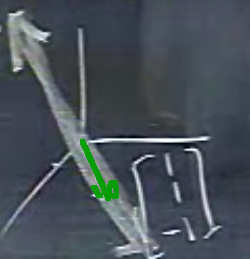
\includegraphics[height=4cm]{6_02.png}

[Yesil ok $\left[\begin{array}{rrr}1 & 1 & -1\end{array}\right]^T$ ve tum
cizgi onun katlari]. Yani sifir uzayi $\mathbb{R}^3$'de bir cizgidir. 

Peki bu sifir uzayi bir alt uzay midir? Bir uzaya ``uzay'' demek sadece
onun belli sartlara uymasi ile mumkundur. Bu sartlar var mi ona bakalim.

$Av=0$ ise ve $Aw=0$ ise, o zaman $A(v+w)=0$ olmali, yani $v$ sifir
uzayinda ise, $w$ sifir uzayinda ise, $v+w$ de sifir uzayinda olmali. Ispat
son derece basit, 

$$ A(v+w) = 0 $$

$$ Av + Aw = 0 $$

ki $Av=0$ ve $Aw=0$ oldugunu biliyorum, o zaman 

$$ \cancelto{0}{Av} + \cancelto{0}{Aw} = 0 + 0 = 0 $$

Bu ispat tamam. Simdi 2. kontrol; sabitle carpim sifir uzayinda midir? 

$$ Ax = 0  $$

$$ A(c \cdot x) = 0  = c \cdot Ax = 0 = c \cdot \cancelto{0}{Ax} = 0$$

Bu sart da yerine getirildi. 

Simdi, karsilastirma amacli olarak, sifir uzayi olmayan bir ornege bakalim,

$$ A = 
\left[\begin{array}{rrr}
1 & 1 & 2 \\
2 & 1 & 3 \\
3 & 1 & 4 \\
4 & 1 & 5 
\end{array}\right]
\left[\begin{array}{r}
x_1  \\
x_2  \\
x_3  
\end{array}\right] 
=
\left[\begin{array}{r}
1  \\
2  \\
3  \\
4  
\end{array}\right]
 $$

Bunu cozen $x$'ler bir vektor uzayi olustururlar mi? Cevap hayir. Bunu
gormenin en basit yolu, sifir vektorunun cozum olmadiginin
gormektir. Sifir vektoru yoksa orijin yok demektir, orijin yoksa bir uzay
elde edemeyiz. 

Bir cozume bakalim, $x = \left[\begin{array}{rrr}
     1&0&0 \end{array}\right]^T$. Digeri? $x = \left[\begin{array}{rrr} 0&-1&1 \end{array}\right]^T$

Boyle bir suru cozum var, fakat bunlar bir alt uzay degil.. Buyuk bir
ihtimalle bu cozumler bir cizgi ya da duzlem olusturuyorlar, ama orijinden 
gecmiyorlar. 



\end{document}
